%Template pembuatan proposal skripsi.
\documentclass{jtetiproposalskripsi}

%-----------------------------------------------------------------
%Disini awal masukan untuk data proposal skripsi
%-----------------------------------------------------------------
\titleind{Simulasi Kinerja Jaringan Nirkabel IEEE-802.11a dan IEEE-802.11g Dengan Menggunakan NS-2}

\fullname{NURCAHYO NOVIANTO}

\idnum{1310652010}

\approvaldate{13 Januari 2030}

\degree{Sarjana Teknik Informatika}

\yearsubmit{2015}

\program{Teknik Informatika}

\dept{Teknik Informatika}


%-----------------------------------------------------------------
%Disini akhir masukan untuk data proposal skripsi
%-----------------------------------------------------------------

\begin{document}

\cover

\approvalpage

%-----------------------------------------------------------------
%Disini akhir masukan untuk muka skripsi
%-----------------------------------------------------------------

%-----------------------------------------------------------------
%Disini awal masukan Intisari
%-----------------------------------------------------------------
\begin{abstractind}
Jaringan nirkabel merupakan jaringan yang menggunakan media transmisi berbasis gelombang radio. Jaringan jenis ini banyak digunakan karena efisiensi dan kemudahan mobilitasnya dalam pertukaran data. Pada penelitian ini dilakukan pemodelan dan simulasi jaringan nirkabel yang mengacu pada spesifikasi teknis perangkat Cisco Aironet 1130ag dengan standar IEEE 802.11a dan IEEE 802.11g. Pemodelan dan simulasi dilakukan dengan perangkat lunak Network Simulator versi 2 (NS-2) yang diinstal pada sistem operasi Linux Ubuntu v.10.10.

Perangkat lunak NS-2 banyak digunakan dan bekerja baik dalam berbagai jenis simulasi jaringan. Dari simulasi didapatkan parameter kualitas layanan jaringan (QoS) dengan menerapkan beberapa skenario simulasi seperti jumlah nodal, jarak antar nodal, serta ukuran paket data. Dari hasil simulasi dapat disimpulkan jaringan dengan standar IEEE 802.11g mempunyai kualitas pengiriman data lebih baik dibanding jaringan dengan standar IEEE 802.11a. Jaringan dengan standar IEEE 802.11g memberikan tingkat performansi rata-rata throughput yang lebih besar dengan nilai rata-rata delay dan persentase packet loss yang lebih kecil dibandingkan dengan hasil simulasi menggunakan jaringan IEEE 802.11a.


\bigskip
\textbf{Kata kunci} : \emph{Wireless Sensor Network}, \emph{Internet Protokol}, WiFi, Network Simulator versi 2, Kualitas Layanan Jaringan, Quality of Services (QoS).
\end{abstractind}
%-----------------------------------------------------------------
%Disini akhir masukan Intisari
%-----------------------------------------------------------------

\tableofcontents
\addcontentsline{toc}{chapter}{DAFTAR ISI}
\selectlanguage{bahasa}\clearpage\pagenumbering{arabic}\setcounter{page}{1}

%-----------------------------------------------------------------
%Disini awal masukan untuk Bab
%-----------------------------------------------------------------
\chapter{LATAR BELAKANG}

\section{Latar Belakang Masalah}
Berbagai macam fasilitas teknologi telekomunikasi terus dikembangkan agar pengguna dapat melakukan komunikasi suara, data, grafik ataupun gambar dengan mudah seiring perkembangan jaringan telekomunikasi dewasa ini mengalami kemajuan yang sangat cepat. Kebutuhan akan komunikasi grafik dan gambar membutuhkan kecepatan data yang semakin tinggi sehingga harus didukung oleh sistem yang handal agar dapat memberikan kualitas layanan dengan baik. Di masa depan jaringan telekomunikasi, lalu lintas dengan kebutuhan performansi yang berbeda akan digabungkan dalam lapis fisik yang sama sehingga akan memerlukan arsitektur jaringan baru yang dapat beradaptasi dengan teknologi ini.

Untuk itu jaringan \textit{\textbf{Optical Burst-Switched}} diusulkan karena dapat menyesuaikan jenis trafik yang dinamis dengan lebih efisien dengan cara mengumpulkan paket pada tepi network. Inovasi di dalam teknologi telekomunikasi berkembang dengan cepat dan selaras dengan perkembangan karakteristik masyarakat modern yang memiliki mobilitas tinggi, mencari layanan yang fleksibel, serba mudah dan memuaskan serta mengejar efisiensi di segala aspek.

\section{Tujuan Penelitian}
Tujuan penelitian ini adalah mempelajari proses, kualitas dan hasil akhir pengiriman data antara standar IEEE 802.11g dengan standar IEEE 802.11a.

\section{Manfaat Penelitian}
Dari hasil simulasi tersebut, dapat disimpulkan jaringan dengan standar IEEE 802.11g mempunyai kualitas pengiriman data lebih baik dibanding jaringan dengan standar IEEE 802.11a. Jaringan dengan standar IEEE 802.11g memberikan tingkat performansi rata-rata throughput yang lebih besar dengan nilai rata-rata delay dan persentase packet loss yang lebih kecil dibandingkan dengan hasil simulasi menggunakan jaringan IEEE 802.11a.

%-------------------------------------------------------------------------------
\chapter{TINJAUAN PUSTAKA DAN DASAR TEORI}                

\section{Tinjauan Pustaka}
Teknologi nirkabel menjadi area yang paling berkembang di bidang jaringan dan telekomunikasi. Jaringan dengan teknologi tersebut dapat mempertukarkan suara, data, dan video. Teknologi nirkabel mempunyai keunggulan diantaranya biaya pembangunan yang relatif murah, instalasi mudah serta kemampuannya menjangkau area geografis yang lebih luas. 
Wireless Fidelity (Wi-Fi) sebagai merk dagang dari aliansi Wi-Fi menjadi teknologi nirkabel yang paling banyak digunakan pada saat ini. Secara teknis Wi-Fi mengacu pada standar komunikasi IEEE 802.11 untuk Wireless Local Area Networks (WLAN). 

Dengan meningkatnya penggunaan jaringan berbasis IEEE 802.11, menjadi sangat penting untuk mengetahui karakteristik trafik jaringan tersebut. Efisiensi dalam pengelolaan jaringan nirkabel menjadi hal yang penting di dalam pengembangan dan pembangunan infrastruktur jaringan. Untuk mengetahui perilaku dan kinerja jaringan nirkabel dapat dilakukan dengan cara pemodelan dan simulasi berdasarkan spesifikasi dan parameter dari komponen-komponen yang menyusun jaringan tersebut. Pemodelan dan simulasi merupakan metode terapan dan eksperimen yang bertujuan untuk menggambarkan perilaku sistem dan memprediksikan perilaku di masa depan dikarenakan ada perubahan di dalam sistem. Tujuan penelitian ini adalah mengetahui kinerja jaringan nirkabel dengan melihat beberapa parameter kualitas layanan jaringan seperti throughput, packet loss, dan delay melalui pemodelan dan simulasi. Selanjutnya juga akan dilihat perbandingan kinerja jaringan yang menggunakan protokol IEEE 802.11a dengan jaringan IEEE 802.11g.

\section{Landasan Teori}
\subsection{\emph{Jaringan Nirkabel}}
Jaringan nirkabel berperan penting dalam pertukaran informasi antar pihak yang tidak tersambung secara fisik. Beberapa jenis jaringan nirkabel yang banyak digunakan adalah bluetooth, Wi-Fi, dan wimax. Institute of Electrical and Electronics Engineering (IEEE) merupakan suatu organisasi yang mengembangkan standar dan aturan untuk aliran komunikasi data pada jaringan nirkabel. Dengan menggunakan standar yang sama, maka suatu perangkat nirkabel dapat berkomunikasi dengan perangkat nirkabel lainnya. Keluarga protokol IEEE 802.11 atau disebut juga Wi-Fi merupakan standar protokol yang paling banyak digunakan pada jaringan WLAN. Tiga standar yang paling banyak diimplementasikan pada banyak perangkat nirkabel LAN adalah IEEE 802.11a, 802.11b, dan 802.11g.

Perbandingan kinerja jaringan antara standar IEEE 802.11a dan IEEE 802.11g menjadi fokus penelitian ini, sehingga pembahasan selanjutnya akan difokuskan pada kedua protokol tersebut. Standar IEEE 802.11a merupakan standar protokol yang menggunakan modulasi \textit{\textbf{Orthogonal Frequency Division Multiplexing}} (OFDM) dan mempunyai laju data maksimum sampai dengan 54 Mbps dengan throughput maksimum sampai 27 Mbps. Standar IEEE 802.11a beroperasi di Industrial, Scientific and Medical (ISM) band antara 5.745 dan 5.805 GHz, dan di bagian \textit{Unlicensed National Information Infrastructure} (UNII) band antara 5.150 GHz dan 5.320 GHz. Dengan frekuensi kerja yang lebih tinggi menyebabkan standar IEEE 802.11a mempunyai jangkauan yang lebih pendek dibandingkan IEEE 802.11b/g dengan daya pancar yang sama. Sedangkan standar IEEE 802.11g juga menggunakan modulasi OFDM dan mempunyai laju data maksimum sampai dengan 54 Mbps dengan throughput maksimum sampai dengan 22 Mbps. 802.11g bekerja pada frekuensi antara 2.400 sampai dengan 2.4835 GHz.


\subsection{Quality of Service (QoS)}
Quality of service (QoS) menunjukkan kemampuan sebuah jaringan dalam menyediakan layanan yang lebih baik bagi trafik yang melewatinya. Beberapa parameter QoS yang dilihat untuk menentukan kualitas suatu jaringan adalah throughput, delay, dan packet loss.

Throughput, dinyatakan dalam satuan bits per second (bps), diukur dengan cara menghitung jumlah paket data yang terkirim secara sukses dalam suatu satuan waktu. Perhitungan throughput hanya memperhitungkan data aktual (payload) yang dikirimkan, tidak memperhitungkan frame header yang mungkin disisipkan selama proses pengiriman paket data.

Sementara delay atau waktu tunda merupakan waktu yang dibutuhkan paket untuk dikirimkan secara sukses dari pengirim ke penerima.

Packet loss adalah presentase jumlah paket yang gagal dikirimkan secara sukses ke tujuan. Kegagalan tersebut dapat diakibatkan oleh berbagai faktor, seperti pelemahan kekuatan sinyal saat proses transmisi, paket yang rusak, kegagalan perangkat jaringan, kegagalan perutean (routing), dan sebagainya.


\subsection{Network Simulator-2 (NS-2)}
Network Simulator-2 (NS-2) merupakan perangkat lunak simulator jaringan bersifat kejadian diskrit dan berorientasi objek, yang dikembangkan oleh UC Berkeley dan USC ISI sebagai bagian dari VINT project. Pada awalnya NS-2 digunakan untuk simulasi jaringan berbasis kabel pada LAN dan WAN, tetapi kemudian dikembangkan sehingga dapat menyimulasikan jaringan nirkabel dan ad-hoc. NS-2 banyak dipergunakan karena sederhana dan bersifat modular.

Skenario simulasi diimplementasikan dalam bentuk skrip simulasi yang ditulis dalam bahasa pemrograman tool command language (tcl). Selain skenario simulasi, tcl juga berisi konfigurasi serta spesifikasi jaringan yang akan disimulasikan. Fleksibilitas NS-2 dapat meningkatkan lingkungan simulasi sesuai dengan yang dibutuhkan, walaupun sebagian besar komponen dasarnya sudah tersedia, seperti komponen nodal baik kabel dan nirkabel, model pola trafik, dan model error.

Hasil simulasi NS-2 dapat berbentuk log file dengan format trace file (.tr), yang berisikan informasi detil paket selama simulasi. Trace file tersebut digunakan oleh Network Animator (NAM), sebuah perangkat visualisasi simulasi yang juga merupakan bagian dari distribusi perangkat lunak NS-2, untuk ditampilkan dalam bentuk animasi simulasi pada layar. Sementara untuk mendapatkan data kuantitas kinerja jaringan seperti throughput, delay dan packet loss, trace file kemudian dibaca oleh perangkat lunak pengolah kata AWK.

%-------------------------------------------------------------------------------

\chapter{METODOLOGI}

\section{Langkah}
Langkah awal untuk melakukan simulasi pada NS-2 adalah membuat file skrip simulasi tcl yang berisikan spesifikasi komponen yang akan digunakan dan kejadian yang seharusnya terjadi. Nilai-nilai parameter yang digunakan disesuaikan dengan karaktersitik perangkat yang sebenarnya. Secara umum, sebuah skenario simulasi terdiri dari tiga komponen, yaitu

\vspace{-0.5cm}

\begin{enumerate}[a.]
\begin{singlespace}
\itemsep0em
\item Topologi jaringan,
\item Koneksi, trafik dan protocol,
\item Kejadian dan kesalahan.
\end{singlespace}
\end{enumerate}


\section{Langkah Kerja}
Pada penelitian ini dilakukan dengan skenario sebagai berikut :

Topologi jaringan yang dibuat diilustrasikan seperti pada gambar 4.1 dengan 1 buah base station dan beberapa mobile station. Simulasi dilakukan untuk beberapa skenario dengan mem-variasikan jumlah node mobile station, jarak antara node base station dengan mobile station, ukuran paket data, dengan protokol komunikasi yang digunakan adalah standar IEEE 802.11a dan IEEE 802.11g

\begin{figure}[ht!]
  \centering
    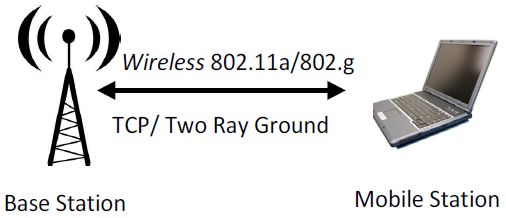
\includegraphics{gambar/1-1}
    \caption{Topologi Jaringan Simulasi}
    \label{Topologi Jaringan Simulasi}
\end{figure}

Satu buah node base station yang digunakan pada jaringan simulasi mengacu pada perangkat Cisco Aironet 1130AG. Sehingga beberapa aspek dan parameter yang digunakan disesuaikan dengan parameter yang ada pada perangkat ini.

\begin{figure}[ht!]
  \centering
    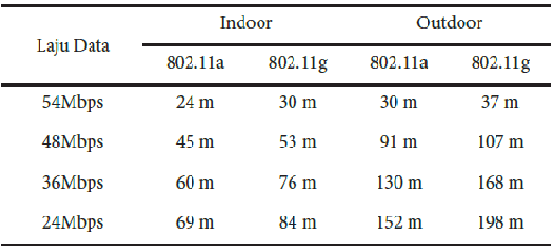
\includegraphics[width=13cm]{gambar/2-1}
\end{figure}
\vspace{-0.2cm}
\begin{center}
Tabel 3.1. Tabel Laju data tergantung pada jarak kedua node.
\end{center}


Protokol perutean yang digunakan dalam simulasi ini yaitu \textit{\textbf{Ad-hoc On-demand Distance Vector}} (AODV) adalah suatu protokol pe-rute-an di jaringan ad-hoc yang bersifat reaktif yang hanya menerima sebuah rute saat dibutuhkan. Node berkomunikasi secara nirkabel dengan model propagasi two ray ground dengan model antena omnidirectional dengan tinggi 1.5 m dan daya penguatan (gain) 3.0 dBi untuk IEEE 802.11g dan 4.5 dBi pada IEEE 802.11a. FTP server digunakan sebagai pembangkit data simulasi dengan menggunakan TCP. Frekuensi tengah kanal sebesar 2.472 MHz pada IEEE 802.11g dan 5 MHz pada IEEE 802.11a. Ukuran paket yang dikirimkan dari mobile station ke base station yaitu 256, 512, dan 1024 bytes. Jarak dari node base station ke masing-masing mobile station divariasikan mulai dari 37 m, 50 m, 100 m, dan 150 m. Laju data akan berubah bergantung dari jarak antara node base station dan mobile station yang berkomukasi mengikuti spesifikasi Cisco Aironet 1130AG (lihat Tabel 1). Untuk collision threshold bernilai 10, dengan nilai carrier sense power disesuaikan dengan spesifikasi Cisco Aironet 1130 AG (lihat gambar tabel). Receive power threshold untuk model propagasi two ray ground ditentukan berdasarkan persamaan berikut :

\textbf{\textit{Dimana, ht dan hr adalah tinggi antena pengirim dan penerima yang dipisahkan dengan jarak d. Pt adalah daya yang ditransmisikan, Gt dan Gr adalah penguatan (gain) perangkat pengirim dan penerima dan L adalah faktor rugi-rugi (loss factor) yang diasumsikan bernilai 1.}}

\begin{figure}[ht!]
  \centering
    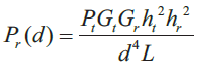
\includegraphics{gambar/3-1}
    \caption{Carrier Sense Power}
    \label{Carrier Sense Power}
\end{figure}
\vspace{-0.5cm}
\begin{figure}[ht!]
  \centering
    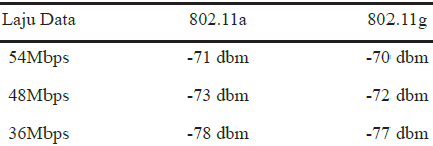
\includegraphics{gambar/3-2}
    \caption{Laju Data}
    \label{Laju Data}
\end{figure}

\section{Hasil dan Pembahasan}
Simulasi dilakukan dengan mem-variasikan jumlah node mobile sebanyak 1 sampai dengan 8 node. Node mobile tersebut masing-masing mengirim paket dengan ukuran 256 byte, 512 byte dan 1024 byte ke nodal base station. Jarak antara node mobile station dengan base station ditentukan yaitu 37 m, 50 m, 100 m, dan 150 m. Dari hasil simulasi didapatkan parameter QoS untuk melihat perbandingan kinerja jaringan IEEE 802.11a dan IEEE 802.11g. Gambar 2 memperlihatkan parameter QoS sebagai fungsi jumlah node mobile station untuk paket dengan ukuran 256 byte. Hasil simulasi tersebut menunjukkan bahwa kinerja jaringan dengan standar IEEE 802.11g lebih baik dibandingkan dengan IEEE 802.11a. Hal ini ditunjukkan dengan nilai rata-rata throughput yang lebih tinggi, tetapi dengan packet loss dan delay yang lebih rendah.

Pada gambar \ref{Hasil Simulasi Jaringan} juga memperlihatkan bahwa penambahan jumlah node mobile station pada jaringan tidak terlalu mempengaruhi throughput. Sementara packet loss dan delay sangat dipengaruhi oleh jumlah nodal mobile di jaringan seperti terlhat pada gambar \ref{Packet Loss} dan \ref{Delay}. Seiring dengan penambahan jumlah user yang diwakili dengan banyaknya nodal mobile station menyebabkan lalu lintas trafik paket data yang lebih padat hal ini ditunjukkan dengan semakin tingginya persentase hilangnya paket (packet loss) dan semakin lamanya paket sampai di tujuan (delay). Perubahan packet loss dan delay pada jaringan IEEE 802.11g seiring penambahan user tidak sebesar pada IEEE 802.11a, hal ini dapat diartikan bahwa jaringan IEEE 802.11g mempunyai kinerja lebih baik dalam menangani banyak user dibanding IEEE 802.11a.

\begin{figure}[ht!]
  \centering
    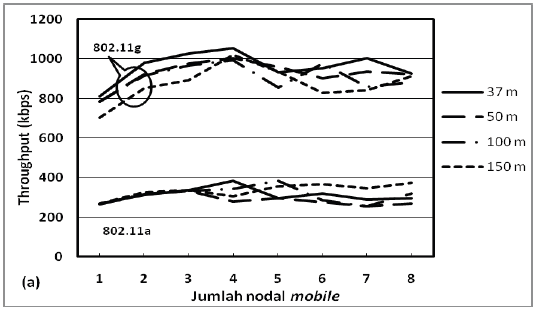
\includegraphics{gambar/2a}
    \caption{Hasil Simulasi Jaringan}
    \label{Hasil Simulasi Jaringan}
\end{figure}
\vspace{-0.5cm}
\begin{figure}[ht!]
  \centering
    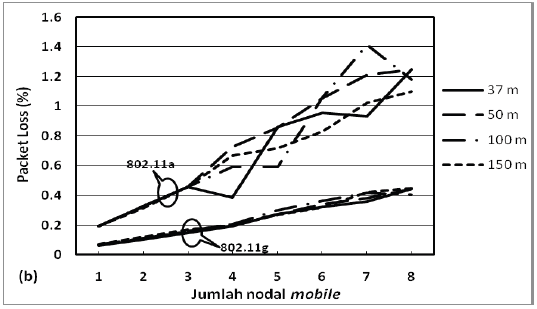
\includegraphics{gambar/2b}
    \caption{Packet Loss}
    \label{Packet Loss}
\end{figure}
\vspace{-0.5cm}
\begin{figure}[ht!]
  \centering
    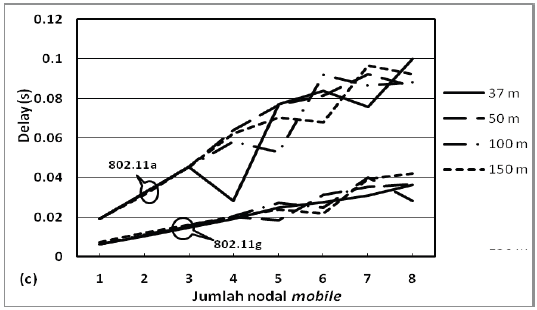
\includegraphics{gambar/2c}
    \caption{Delay sebagai fungsi jumlah node mobile station dengan masing-masing jarak ke base station adalah 37 m, 50 m, 100 m, dan 150 m}
    \label{Delay}
\end{figure}

\begin{figure}[ht!]
  \centering
    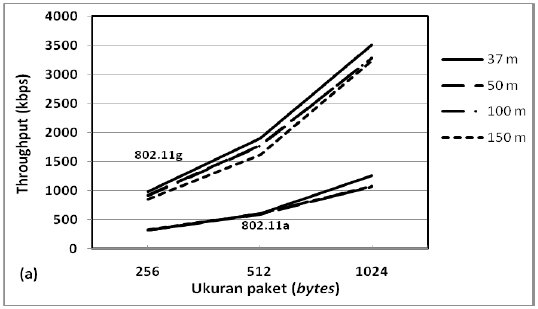
\includegraphics{gambar/4a}
    \caption{Hasil simulasi jaringan untuk throughput}
    \label{Hasil simulasi jaringan untuk throughput}
\end{figure}

\begin{figure}[ht!]
  \centering
    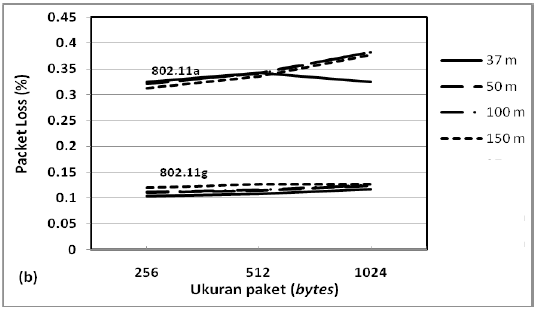
\includegraphics{gambar/4b}
    \caption{Packet Loss}
    \label{PacketLoss}
\end{figure}

\begin{figure}[ht!]

  \centering
    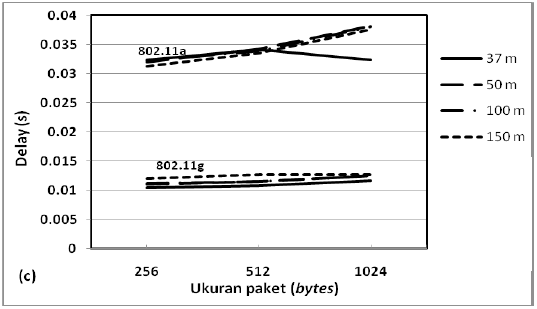
\includegraphics{gambar/4c}
    \caption{Delay sebagai fungsi ukuran paket yang dikirimkan dengan jarak base station ke masing-masing mobile station adalah 37 m, 50 m, 100 m dan 150 m}
    \label{Delay sebagai}
\end{figure}

Parameter QoS juga digambarkan sebagai fungsi dari ukuran paket (dalam byte), seperti yang ditunjukkan pada Gambar 3. Dari gambar tersebut memperlihatkan parameter QoS untuk simulasi jaringan dengan 1 base station dan 2 mobile station dengan jarak base station ke masing-masing mobile station 37 m, 50 m, 100 m, dan 150 m serta ukuran paket divariasikan mulai 256, 512, dan 1024 btye.

Seperti yang sudah diperkirakan, kinerja jaringan standar IEEE 802.11g lebih baik dari IEEE 802.11a. Hal ini ditunjukkan dari perbandingan rata-rata throughput, packet loss dan delay untuk kedua jaringan tersebut. Seiring dengan kenaikan ukuran paket yang dikirimkan terlihat bahwa rata-rata throughput yang terukur mengalami kenaikan seperti terlihat pada \ref{Hasil simulasi jaringan untuk throughput}. Hanya pada jaringan dengan standar IEEE 802.11g mempunyai kecendrungan kenaikan yang lebih tinggi dibanding jaringan dengan IEEE 802.11a. Sementara itu ukuran paket tidak terlalu mempengaruhi packet loss dan delay yang terjadi. Pada \ref{PacketLoss} dan \ref{Delay sebagai} memperlihatkan nilai packet loss dan delay yang relatif konstan dengan perubahan ukuran paket yang dikirimkan.

Naskah ini memaparkan perbandingan kinerja jaringan dengan protocol IEEE 802.11a dan IEEE 802.11g. Hasil simulasi menunjukkan bahwa kinerja jaringan dengan standar IEEE 802.11g lebih baik dibanding dengan IEEE 802.11a, hal ini terlihat dari nilai rata-rata throughput yang lebih besar serta nilai packet loss dan delay yang lebih kecil. Ini terjadi pada simulasi jaringan baik dengan memvariasikan jumlah nodal mobile atau ukuran paket data yang dikirimkan. 
Simulasi jaringan dengan memvariasikan jumlah nodal mobile station (pengguna), terlihat bahwa walaupun rata-rata throughput relatif stabil, tetapi lalu lintas trafik paket data semaikn padat yang ditunjukkan dengan semakin tingginya persentase hilangnya paket (packet loss) dan semakin lamanya paket sampai di tujuan (delay). Selanjutnya, simulasi jaringan dengan memvariasikan jumlah nodal mobile station (pengguna) juga terlihat bahwa perubahan packet loss dan delay pada jaringan IEEE 802.11g tidak sebesar pada IEEE 802.11a, hal ini dapat diartikan bahwa jaringan IEEE 802.11g mempunyai kinerja lebih baik dalam menangani lebih banyak pengguna dibanding IEEE 802.11a. Sementara simulasi jaringan dengan memvariasikan ukuran paket, dapat terlihat bahwa packet loss dan delay tidak terlalu terpengaruh dibanding pada perubahan jumlah mobile station (pengguna).

%-----------------------------------------------------------------
%Disini akhir masukan Bab
%-----------------------------------------------------------------

%-----------------------------------------------------------------
%Disini awal masukan untuk Daftar Pustaka
%-----------------------------------------------------------------
%%\nocite{Abel2010,Guerbas201350}
%%\bibliography{research-plan}
%%\bibliographystyle{plainnat}
\begin{thebibliography}{9}

\bibitem[satu(2013)]{satu01}
W, Stallings, Wireless Communications and Networks , Prentice Hall, 2005

\bibitem[dua(2013)]{dua02}
R. E. Shannon, “Introduction to the Art and Science of Simulation,” in Proceedings of Winter Simulation Conference, 1988

\bibitem[tiga(2013)]{tiga03}
Information technology, Telecommunications and Information Exchange Between Systems Local and Metropolitan Area Networks  Specific Requirements, Wireless LAN Medium Access Control (MAC) and Physical Layer (PHY) specifications; IEEE Standard 802.11, 1999

\bibitem[empat(2013)]{empat04}
Telecommunications and Information Exchange Between Systems Local and Metropolitan Area Networks, Specific Requirements Part 11: Wireless LAN Medium Access Control (MAC) and Physical Layer (PHY) specifications, IEEE Standard 802.11g, 2003.

\bibitem[lima(2013)]{lima05}
Network Simulator [Online], Avalaible on www.isi.edu/nsnam/ns/

\bibitem[enam(2013)]{enam06}
B. Welch, Practical Programming in Tcl and Tk, Prentice Hall, 1995

\bibitem[tujuh(2013)]{tujuh07}
A. D. Robbins, GAWK: Effective AWK Programming, Boston, MA: Free Software Foundation, 2009.

\bibitem[tujuh(2013)]{delapan08}
Cisco Aironet 1130AG Data Sheet [Online]. Avalable: http://www.cisco.com/.

\bibitem[tujuh(2013)]{sembilan09}
C. E. Perkins and E. M. Royer, “Adhoc on demand distance vector routing,” in Proceeding 2nd IEEE Workshop on Mobile Computer Systems and Applications, 1999, pp. 90-100.

\end{thebibliography}
\addcontentsline{toc}{chapter}{DAFTAR PUSTAKA}
%-----------------------------------------------------------------
%Disini akhir masukan Daftar Pustaka
%-----------------------------------------------------------------

\end{document}
